La compression de graphes est définie comme l'ensemble des méthodes et techniques permettant de réduire l'espace mémoire occupé par ce derniers tout en gardant la même signification que le graphe d'origine. Dès lors, deux approches se présentent: la compression avec ou sans perte, que nous allons détailler dans ce qui suit.
			
			\begin{enumerate}[label=\alph*)]
			\item \subsubsection{Compression Sans Perte:}
			Certains domaines d'application de la compression nécessitent un niveau élevé d'exactitude et une restitution exacte, donc une compression sans perte. Dans cette catégorie, le graphe G subit des transformations pour avoir une représentation compacte $G'$ qui lors de la décompression donne exactement G. La figure ci-dessous illustre cette définition. 
			
			\begin{figure}[h]
			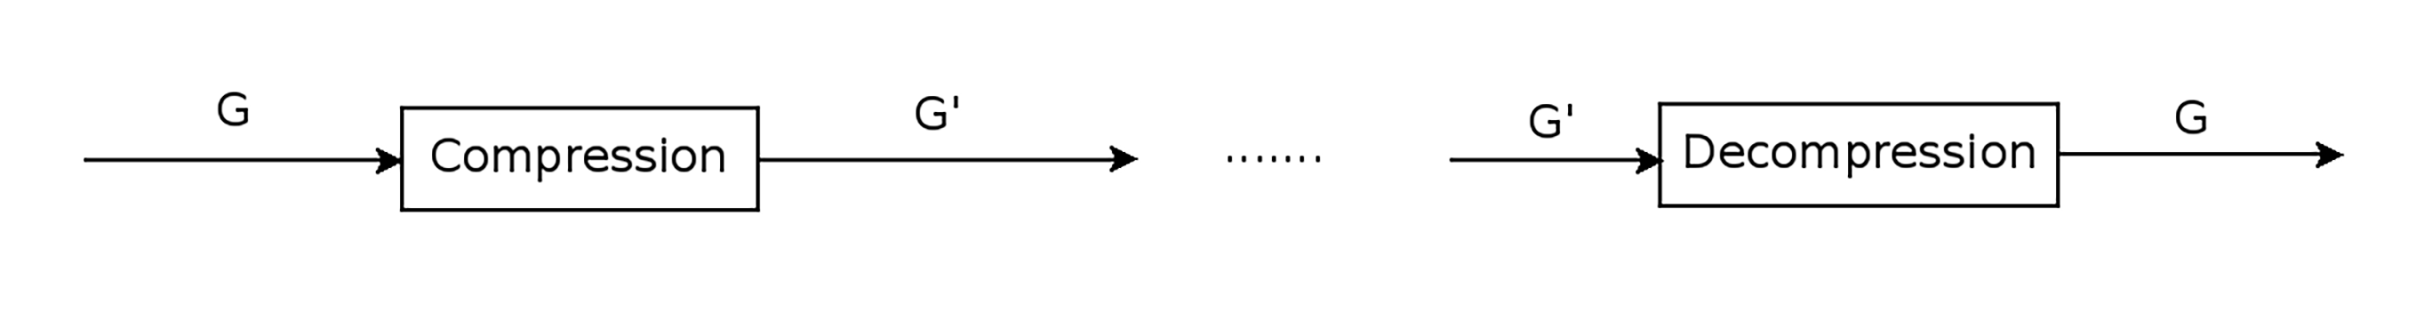
\includegraphics[scale=0.15,center]{./ressources/image/SansPerte.png}
			\caption[Compression sans perte.]{Compression sans perte.}
			\end{figure}
			
			%% citee qlq exemple de compression sans pertes
			
			\item \subsubsection{Compression Avec Perte:}
			Contrairement à la compression sans perte, la compression avec perte permet la suppression permanente de certaines informations jugées inutiles (redondantes) pour améliorer la qualité de la compression.  En d'autres termes, le graphe G subit des transformations pour avoir une représentation compacte $G'$ qui lors de la décompression donne un graphe $G''$ probablement différent de G mais l'approximant le plus possible. La figure ci-dessous illustre cette définition.   
			
			\begin{figure}[h]
			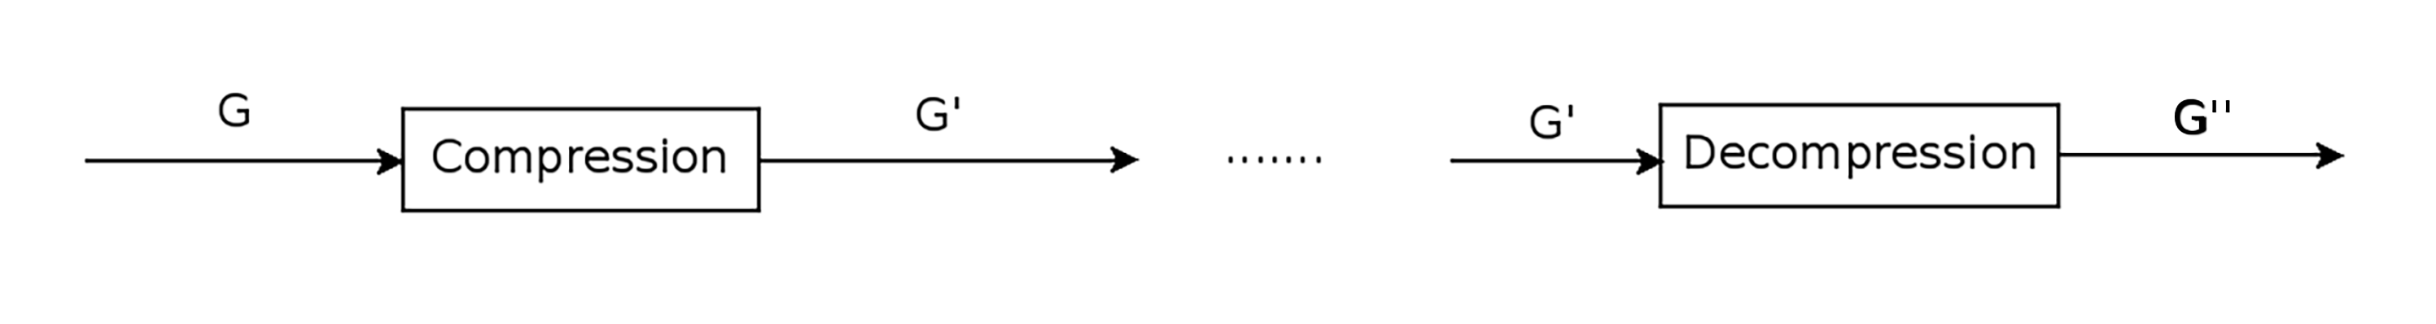
\includegraphics[scale=0.15,center]{./ressources/image/AvecPerte.png}
			\caption[Compression avec perte.]{Compression avec perte.}
			\end{figure}
			
			%%% citee qlq exemple de compression avec perte
				\end{enumerate}
			
			
			